\section{Satisfied\-IND\_\-DBMS$<$ DBMS $>$ Class Template Reference}
\label{class_satisfied_i_n_d___d_b_m_s}\index{SatisfiedIND_DBMS@{SatisfiedIND\_\-DBMS}}
Functor representing the predicate being a satisfied {\bf IND}{\rm (p.\,\pageref{class_i_n_d})} wrt to 2 relations in a SGBD.  


{\tt \#include $<$Satisfied\-IND\_\-DBMS.hxx$>$}

Inheritance diagram for Satisfied\-IND\_\-DBMS$<$ DBMS $>$::\begin{figure}[H]
\begin{center}
\leavevmode
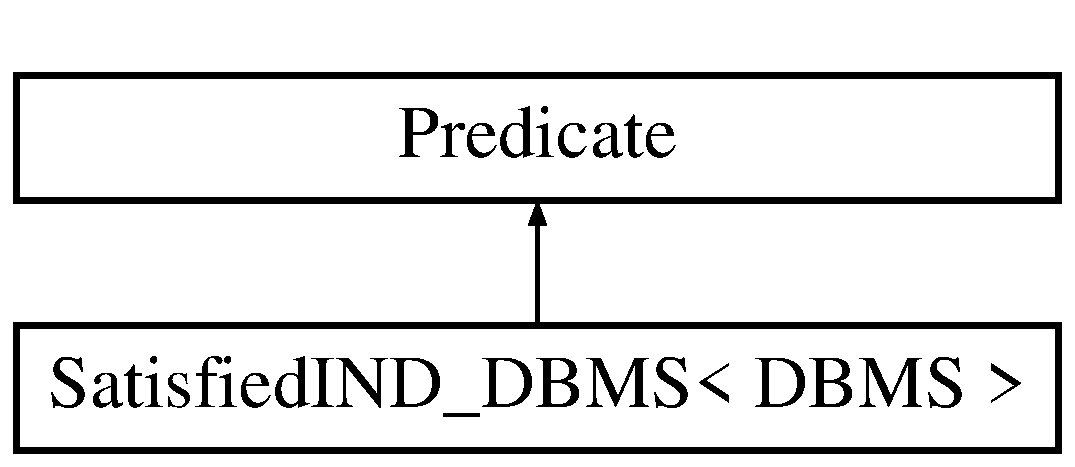
\includegraphics[height=2cm]{class_satisfied_i_n_d___d_b_m_s}
\end{center}
\end{figure}
\subsection*{Public Member Functions}
\begin{CompactItemize}
\item 
{\bf Satisfied\-IND\_\-DBMS} (DBMS $\ast$in\-Dbms)
\begin{CompactList}\small\item\em Constructor. \item\end{CompactList}\item 
{\bf $\sim$Satisfied\-IND\_\-DBMS} ()\label{class_satisfied_i_n_d___d_b_m_s_26071485b5e3be1fb328fe4cc1a9a336}

\begin{CompactList}\small\item\em Destructor. \item\end{CompactList}\item 
template$<$class Iterator, class Measure$>$ bool {\bf operator()} (Iterator it\-Cand, Measure \&mes\-Cand)\label{class_satisfied_i_n_d___d_b_m_s_10cb098e49804f3de10b20c1d3317814}

\begin{CompactList}\small\item\em Operator that test if a set of attributes is not redundant. \item\end{CompactList}\end{CompactItemize}
\subsection*{Protected Attributes}
\begin{CompactItemize}
\item 
DBMS $\ast$ {\bf mydbms}\label{class_satisfied_i_n_d___d_b_m_s_6a69c4a2896c294ee5bb98959f1775bc}

\begin{CompactList}\small\item\em Pointer on the dbms. \item\end{CompactList}\end{CompactItemize}


\subsection{Detailed Description}
\subsubsection*{template$<$class DBMS$>$ class Satisfied\-IND\_\-DBMS$<$ DBMS $>$}

Functor representing the predicate being a satisfied {\bf IND}{\rm (p.\,\pageref{class_i_n_d})} wrt to 2 relations in a SGBD. 

This functor test if a {\bf IND}{\rm (p.\,\pageref{class_i_n_d})} is satisfied for two relation stored in a DBMS. Note that each time the functor is used, a query is executed on the database.

The template parameter DBMS is the class representing the connection to the DBMS. This class is used to do operations on the DBMS such as connect, execute a query ...

The attributes in the two relations must have the same data type. 



\subsection{Constructor \& Destructor Documentation}
\index{SatisfiedIND_DBMS@{Satisfied\-IND\_\-DBMS}!SatisfiedIND_DBMS@{SatisfiedIND\_\-DBMS}}
\index{SatisfiedIND_DBMS@{SatisfiedIND\_\-DBMS}!SatisfiedIND_DBMS@{Satisfied\-IND\_\-DBMS}}
\subsubsection{\setlength{\rightskip}{0pt plus 5cm}template$<$class DBMS$>$ {\bf Satisfied\-IND\_\-DBMS}$<$ DBMS $>$::{\bf Satisfied\-IND\_\-DBMS} (DBMS $\ast$ {\em in\-Dbms})\hspace{0.3cm}{\tt  [inline]}}\label{class_satisfied_i_n_d___d_b_m_s_90330aefbc693768d516a523f4f04625}


Constructor. 

\begin{Desc}
\item[Parameters:]
\begin{description}
\item[{\em in\-Dbms}]pointer on the DBMS and the database studied \end{description}
\end{Desc}


The documentation for this class was generated from the following file:\begin{CompactItemize}
\item 
F:/i\-Zi/problems/DI/Satisfied\-IND\_\-DBMS.hxx\end{CompactItemize}
